\chapter{The Operator Panel}
\label{ch:panel}

The operator panel is the machine's control surface. Every action that moves the machine,
changes the spindle or changes an override starts here. LiNC reads the panel and shows what
it is doing; it never sends those commands.

The panel runs as its own process (\texttt{linc-panel}) and owns the panel link. It
publishes a fixed set of button, lamp, display and override signals to the controller's
HAL, named \halpin{cnc\_panel.*}. The interface reads the same signals. A crash of the
interface therefore does not take the panel away, and the interface never opens the panel
port.

\begin{notebox}
  The interface cannot write a \halpin{cnc\_panel.*} pin. It writes only its own seven
  declared outputs, and \halpin{net-safe} is the only one that reaches machine logic.
\end{notebox}

\shot{img/ui/panel.png}{The simulated operator panel, mill face. A physical panel carries
the same groups; the machine builder decides the exact legends of the machine function
keys.}{fig:panel}

\section{Power and emergency stop}

The power group and the emergency stop are described in chapter~\ref{ch:power}. The panel
is where they are pressed; the screen only reports them.

\section{The mode selector}

\begin{figure}[H]
  \centering
  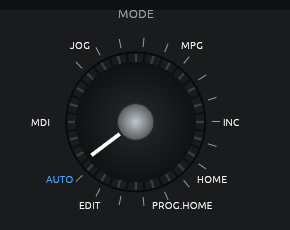
\includegraphics[width=0.44\textwidth]{img/crops/mode.png}
  \caption{The \textbf{MODE} selector. Its eight steady positions are read as one-hot
           signals: exactly one position must be active.}
  \label{fig:mode}
\end{figure}

The selector is read as a steady position, not as pulses. Zero or several active positions
is a fault: LiNC shows \state{PANEL MODE INVALID} and refuses mode-dependent actions.

\begin{longtable}{L{2.5cm}L{4.6cm}L{5.9cm}}
  \toprule
  \textbf{Position} & \textbf{Panel / controller} & \textbf{What LiNC does} \\
  \midrule
  \endhead
  EDIT & Manual mode, editing allowed & Opens Program in the \sbtn{CODE} layout and focuses
         the editor. Saving is allowed only here. \\
  AUTO & Automatic mode & Brings the Machine page forward. Cycle start then belongs to the
         panel. \\
  MDI  & Manual data input & Opens the Machine page with the MDI pane in place of the program
         card. \keycap{Enter} issues the block. \\
  JOG  & Manual mode, continuous jog & Opens the Manual page: live toolpath, coordinates,
         jog context. \\
  INC  & Manual mode, step jog & Same page, with the increment row. The steps come from the
         machine INI. \\
  MPG  & Manual mode, handwheel & Same page; the handwheel selects its own step. \\
  HOME & Manual mode, homing & Opens the Homing page with the machine position and the homing
         state of each axis. \\
  PROG.HOME & Manual mode, program zero & Opens the Homing page titled \state{PROGRAM ZERO}. The
         axis keys send the program-zero blocks, not jogs. \\
  \bottomrule
\end{longtable}

\begin{notebox}
  The selector is authoritative for what the panel keys do. LiNC's own page changes are a
  convenience copy of that state; where the two disagree, the panel wins. The top bar shows
  \state{PANEL} and \state{TASK} separately, so a disagreement is visible.
\end{notebox}

\section{The override knobs}

\begin{figure}[H]
  \centering
  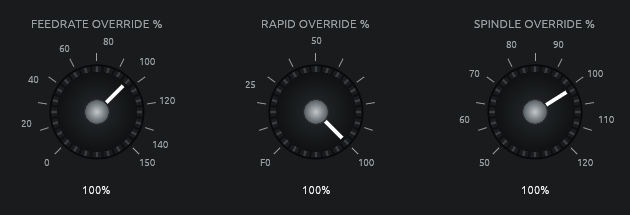
\includegraphics[width=0.86\textwidth]{img/crops/overrides.png}
  \caption{Feedrate, rapid and spindle override. The percentage under each knob is the
           current value; the interface repeats all three in the bottom bar.}
  \label{fig:overrides}
\end{figure}

The three knobs are steady analogue values sampled by the panel service. LiNC displays them
as \state{OVR F100 R100 S100} in the bottom bar, and the Machine page uses the feed and
spindle percentages in its \sbtn{FEED / SPINDLE} card.

\begin{itemize}
  \item \textbf{Feedrate override} scales programmed feed. On the shipped panel it ranges
        from 0 to 150\,\%.
  \item \textbf{Rapid override} scales rapid moves. \texttt{F0} stops rapids.
  \item \textbf{Spindle override} scales the commanded spindle speed. It does not change the
        displayed true speed, which comes from feedback.
\end{itemize}

\begin{cautionbox}
  An override of 0\,\% feed looks like a machine that will not move. Check the knobs before
  diagnosing a fault: the bottom bar always shows them.
\end{cautionbox}

\section{Cycle keys and axis keys}

\begin{figure}[H]
  \centering
  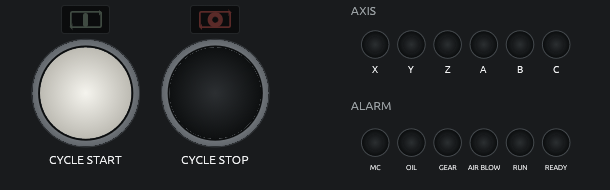
\includegraphics[width=0.77\textwidth]{img/crops/lamps.png}
  \caption{Left: \textbf{CYCLE START} (illuminated white) and \textbf{CYCLE STOP}. Centre: the
           axis lamps. Right: the alarm lamps.}
  \label{fig:cyclekeys}
\end{figure}

\begin{description}[font=\normalfont\sffamily\bfseries, leftmargin=3.1cm, style=nextline]
  \item[\pbtn{CYCLE START}] Starts the loaded program. The controller gates it: machine on,
        no emergency stop, axes homed, interpreter idle, and the panel in AUTO. LiNC does
        not issue it and cannot issue it.
  \item[\pbtn{CYCLE STOP}] Stops the program and stops motion.
  \item[Axis keys] Jog in JOG and INC, home in HOME, and send the program-zero block in
        PROG.HOME, all according to the mode selector and the machine's HAL wiring.
  \item[\pbtn{RAPID}] With an axis key, jogs at rapid rate; in HOME it starts homing all
        axes; in PROG.HOME it sends the all-axes program-zero block.
\end{description}

The axis lamps light for the axes the controller reports. The alarm lamps report machine
conditions (machine ready, run, and the machine's own alarm set). \state{READY} follows
machine power and an idle or paused program.

\section{The displays}

\begin{figure}[H]
  \centering
  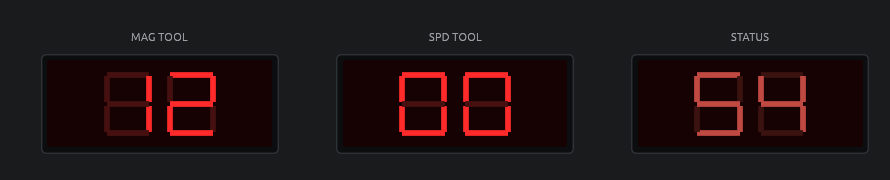
\includegraphics[width=0.95\textwidth]{img/crops/displays.png}
  \caption{The tool displays and the two-digit status display. Here the status display
           shows \texttt{54}, the active work coordinate system.}
  \label{fig:displays}
\end{figure}

\begin{itemize}
  \item \textbf{MAG TOOL} is the tool in the spindle as the controller reports it.
  \item \textbf{SPD TOOL} is the prepared tool, where the machine has a changer.
  \item \textbf{STATUS} shows the active work coordinate system, \texttt{54} to
        \texttt{59}. It shows \texttt{-{}-} when the value is unknown, stale or outside
        those systems, and never a guess.
\end{itemize}

The interface writes \halpin{linc.status-display} and the machine's post-GUI HAL maps it to
the display. This is one of the seven declared outputs.

\section{The machine function keys}

The key matrix carries the machine functions: spindle forward, stop, reverse and orient;
coolant; air blow; chuck; lube; chip conveyor; work lamp; safe door; tool changer and pot
keys; and the four free keys \pbtn{K1} to \pbtn{K4}. Each key is a HAL button; the machine
configuration decides what it switches.

\begin{notebox}
  Only the keys the machine wires do something. A key with no net in the machine's HAL is
  inert, and the simulated panel greys the keys its profile does not wire. Nothing on the
  screen duplicates these functions.
\end{notebox}

\section{The simulated panel}

The simulated panel is a window that speaks the same protocol as a physical panel. It is
used for the simulator, for training and for a machine that has no panel cabinet.

\begin{itemize}
  \item It draws the face the profile selects: mill or lathe, with that face's keys, lamps
        and displays.
  \item It publishes the same \halpin{cnc\_panel.*} signals as the real driver, so the
        interface and the HAL cannot tell the difference.
  \item It starts in the safe state: emergency stop latched, power off.
  \item It runs on a second monitor if you put it there. With no physical panel, a touch
        screen or a mouse can operate it; that makes the pointer a replacement for the
        panel hardware, not a second set of machine controls.
\end{itemize}

The panel window also answers the keyboard, so it can be used without a pointer:

\begin{center}
\begin{tabular}{ll}
  \toprule
  \textbf{Key} & \textbf{Action} \\
  \midrule
  \keycap{P} & Power on (also releases the emergency stop) \\
  \keycap{O} & Power off \\
  \keycap{E} & Press / release the emergency stop \\
  \keycap{R} & Rapid (hold) \\
  \keycap{C} & Cycle start \\
  \keycap{S} & Cycle stop \\
  \keycap{1} \dots \keycap{8} & Mode selector: EDIT, AUTO, MDI, JOG, INC, MPG, HOME, PROG.HOME \\
  \bottomrule
\end{tabular}
\end{center}

\begin{tipbox}
  In a demonstration on one computer, keep the panel window on the second monitor and give
  the interface the first one. The interface's \keycap{F5} to \keycap{F8} keys and the
  panel's number keys act on different windows, so the focus must be where the key belongs.
\end{tipbox}
